\documentclass[lettersize,journal]{IEEEtran}
\usepackage{amsmath,amsfonts}
\usepackage{algorithmic}
\usepackage{array}
\usepackage[caption=false,font=normalsize,labelfont=sf,textfont=sf]{subfig}
\usepackage{textcomp}
\usepackage{stfloats}
\usepackage{url}
\usepackage{verbatim}
\usepackage{graphicx}
\usepackage[UTF8]{ctex}

\def\UrlBreaks{\do\A\do\B\do\C\do\D\do\E\do\F\do\G\do\H\do\I\do\J
\do\K\do\L\do\M\do\N\do\O\do\P\do\Q\do\R\do\S\do\T\do\U\do\V
\do\W\do\X\do\Y\do\Z\do\[\do\\\do\]\do\^\do\_\do\`\do\a\do\b
\do\c\do\d\do\e\do\f\do\g\do\h\do\i\do\j\do\k\do\l\do\m\do\n
\do\o\do\p\do\q\do\r\do\s\do\t\do\u\do\v\do\w\do\x\do\y\do\z
\do\.\do\@\do\\\do\/\do\!\do\_\do\|\do\;\do\>\do\]\do\)\do\,
\do\?\do\'\do+\do\=\do\#}

\usepackage{float}
\usepackage[justification=centering]{caption}

\usepackage{balance}
\begin{document}
\title{数据聚类}
\author{姓名:尹伯豪\ 学号:2112215089}



\maketitle

\begin{abstract}
本文基于交通信号灯数据集GTSRB,采用K-means和Mean Shift聚类方法,从两个视角进行实验分析。首先,将图片处理成相同大小,进行高维聚类。其次,选择一张图片,将其视为RGB空间中的点集,进行基于聚类的图像分割。实验结果展示了聚类效果,并进行了定量和定性的对比分析。通过实验,我们可以深入理解K-means和Mean Shift聚类方法的原理,并评估其在交通信号灯数据集上的效果。
\end{abstract}



\section{方法原理}

聚类方法是一种将数据点分组成相似的集合的技术。下面简述K-means和Mean Shift聚类方法的原理:

1. K-means聚类方法原理

K-means聚类方法的原理是基于距离的聚类算法。它的目标是将数据点分配到K个簇中,使得每个数据点与所属簇的中心点之间的平方距离最小化。其算法步骤如下:

\begin{enumerate}
    \item 选择K个初始聚类中心,可以是随机选择或根据数据分布选择。
    \item 将所有数据点分配到距离最近的聚类中心,形成K个簇。
    \item 更新每个簇的中心点为所属数据点的平均值。
    \item 重复步骤2和步骤3,直到聚类中心不再发生变化或达到预定的迭代次数。
\end{enumerate}

K-means聚类方法通过迭代优化聚类中心位置,使得簇内数据点的相似性最大化,簇间数据点的差异性最大化。

2. Mean Shift聚类方法原理

Mean Shift聚类方法是一种基于密度的聚类算法。它的核心思想是通过寻找数据点密度梯度的极值点来确定聚类中心。其算法步骤如下:

\begin{enumerate}
    \item 选择初始聚类中心,可以是随机选择或根据数据分布选择。
    \item 对于每个聚类中心,计算每个数据点对其的偏移向量,即数据点指向聚类中心的方向和距离。
    \item 将每个数据点根据偏移向量移动到局部密度最大的方向上。
    \item 重复步骤2和步骤3,直到聚类中心不再发生明显的移动或达到预定的迭代次数。
\end{enumerate}

Mean Shift聚类方法通过不断移动数据点,使得数据点向局部密度高的区域聚集,从而确定聚类中心。相比于K-means,Mean Shift聚类方法可以自适应地调整聚类中心的数量。

这两种聚类方法在处理不同数据集和问题时具有各自的特点和适用性。在实验中,我们将使用这两种方法来对交通信号灯数据集进行聚类,并评估其效果。

\section{高维聚类}

首先,为了将图片处理成相同大小,使用了transforms.Resize函数来调整图片的尺寸,将图片的大小调整为32x32像素。每张图片可以被看作是一个数据点,其中每个像素的RGB值可以作为该数据点的特征。在进行聚类之前,可能需要考虑将高维数据进行降维或特征提取。常用的降维方法在上次实验中已经进行过详细介绍,包括主成分分析(PCA)和t-SNE等。这些方法可以将高维特征转换为低维表示,以便更好地可视化和聚类。在这里,我们选择使用PCA来降低数据的维度。

接下来,我们使用两种聚类方法来进行数据聚类:K-means和Mean Shift。K-means是一种常见的基于距离的聚类算法,它将数据点分成预定义数量的簇。Mean Shift是一种非参数化的聚类算法,它通过寻找数据点密度最大的区域来进行聚类。下图是经过PCA降维的K\-means聚类和Mean Shift聚类及其与原始数据对比的可视化展示,

\begin{figure}[H]
\centering
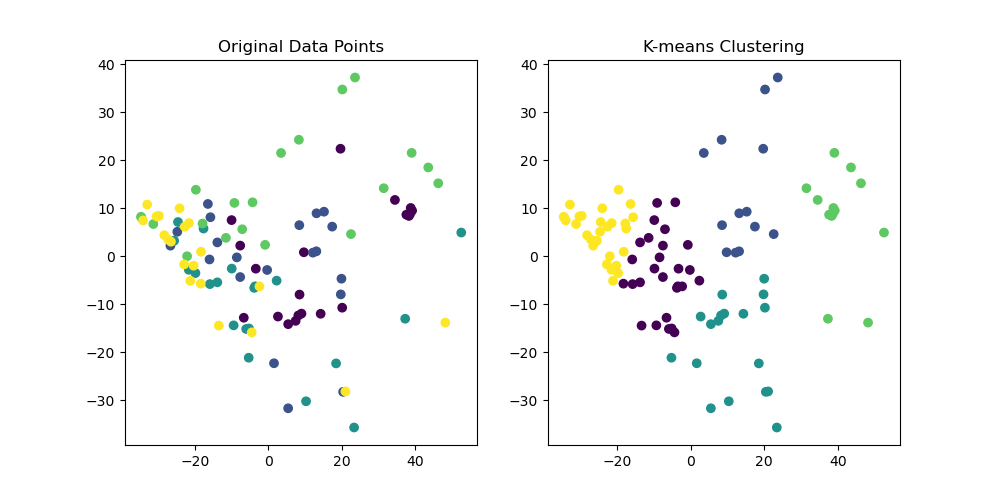
\includegraphics[width=3in]{image/Figure_1.png}
\caption{PCA降维K-means聚类}
\end{figure}

\begin{figure}[H]
\centering
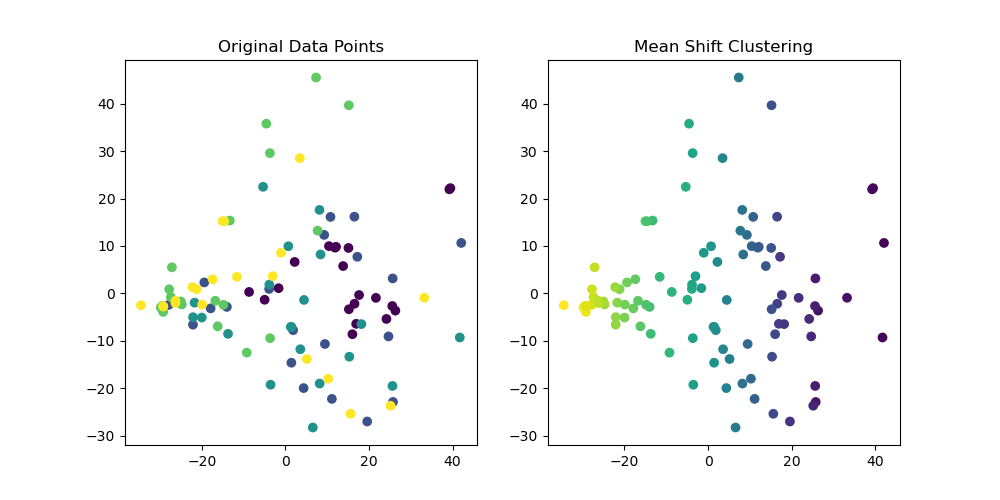
\includegraphics[width=3in]{image/Figure_2.png}
\caption{PCA降维Mean Shift聚类}
\end{figure}

只从可视化图像也可以看出聚类效果不是很好,只能大概的看出分布方向与规模,而从具体的聚类效果来看,本实验采用轮廓系数(Silhouette Score),兰德指数(Adjusted Rand Index,ARI)和准确率(Accuracy)来定量的分析聚类效果,具体输出如下:

K-means Silhouette Score: 0.41785222

Mean Shift Silhouette Score: 0.40998787

ari\_kmeans: 0.08609692288526224

ari\_meanshift: 0.08089161326274728

accuracy\_kmeans: 0.31

accuracy\_meanshift: 0.09

根据输出结果可以看出,

\begin{enumerate}
    \item 轮廓系数越接近1表示聚类效果越好,K-means和Mean Shift的轮廓系数都相对较高,但差距不大。
    \item ARI的取值范围在-1到1之间,值越接近1表示聚类效果越好。根据结果,K-means和Mean Shift的ARI值较低,说明聚类结果与真实标签的一致性较低。
    \item 准确率用于衡量聚类结果与真实标签之间的匹配程度,取值范围为0到1之间。根据结果,K-means的准确率较高,但仍然有提升的空间;而Mean Shift的准确率较低。
\end{enumerate}

根据以上结果分析,当前的聚类效果仍然有改进的空间。接下来可能会考虑尝试不同的聚类算法、特征工程方法和数据预处理方式,或者继续调整聚类算法的参数,以找到更好的聚类方案。除此之外,增加更多的训练样本、扩充数据集以及优化特征选择,可能也会提高聚类的准确性和一致性。




\section{基于聚类的图像分割}

本实验使用K均值聚类算法对图像进行分割,将图像中的像素点聚类为不同的区域,并对每个区域进行可视化展示。

首先,从数据集中随机选取一张图片,转换成数组,使用K均值聚类,获取每个点的聚类标签,并将聚类标签reshape为原始图像形状,打印输出每个聚类的像素数量。为了与原始图像进行对比,创建一个与原始图像相同大小的矩阵来存储分割结果

segmented\_image = np.zeros\_like(image\_array)

接下来为每个聚类设置不同颜色并根据聚类标签对像素点进行着色。最后将结果可视化展示,通过在三维坐标系中绘制点集,其中每个点的坐标表示RGB值,实现对图像的可视化展示。另外,还通过图像显示对比来展示分割结果和原始图像。

K = 3 时结果显示:

\begin{figure}[H]
\centering
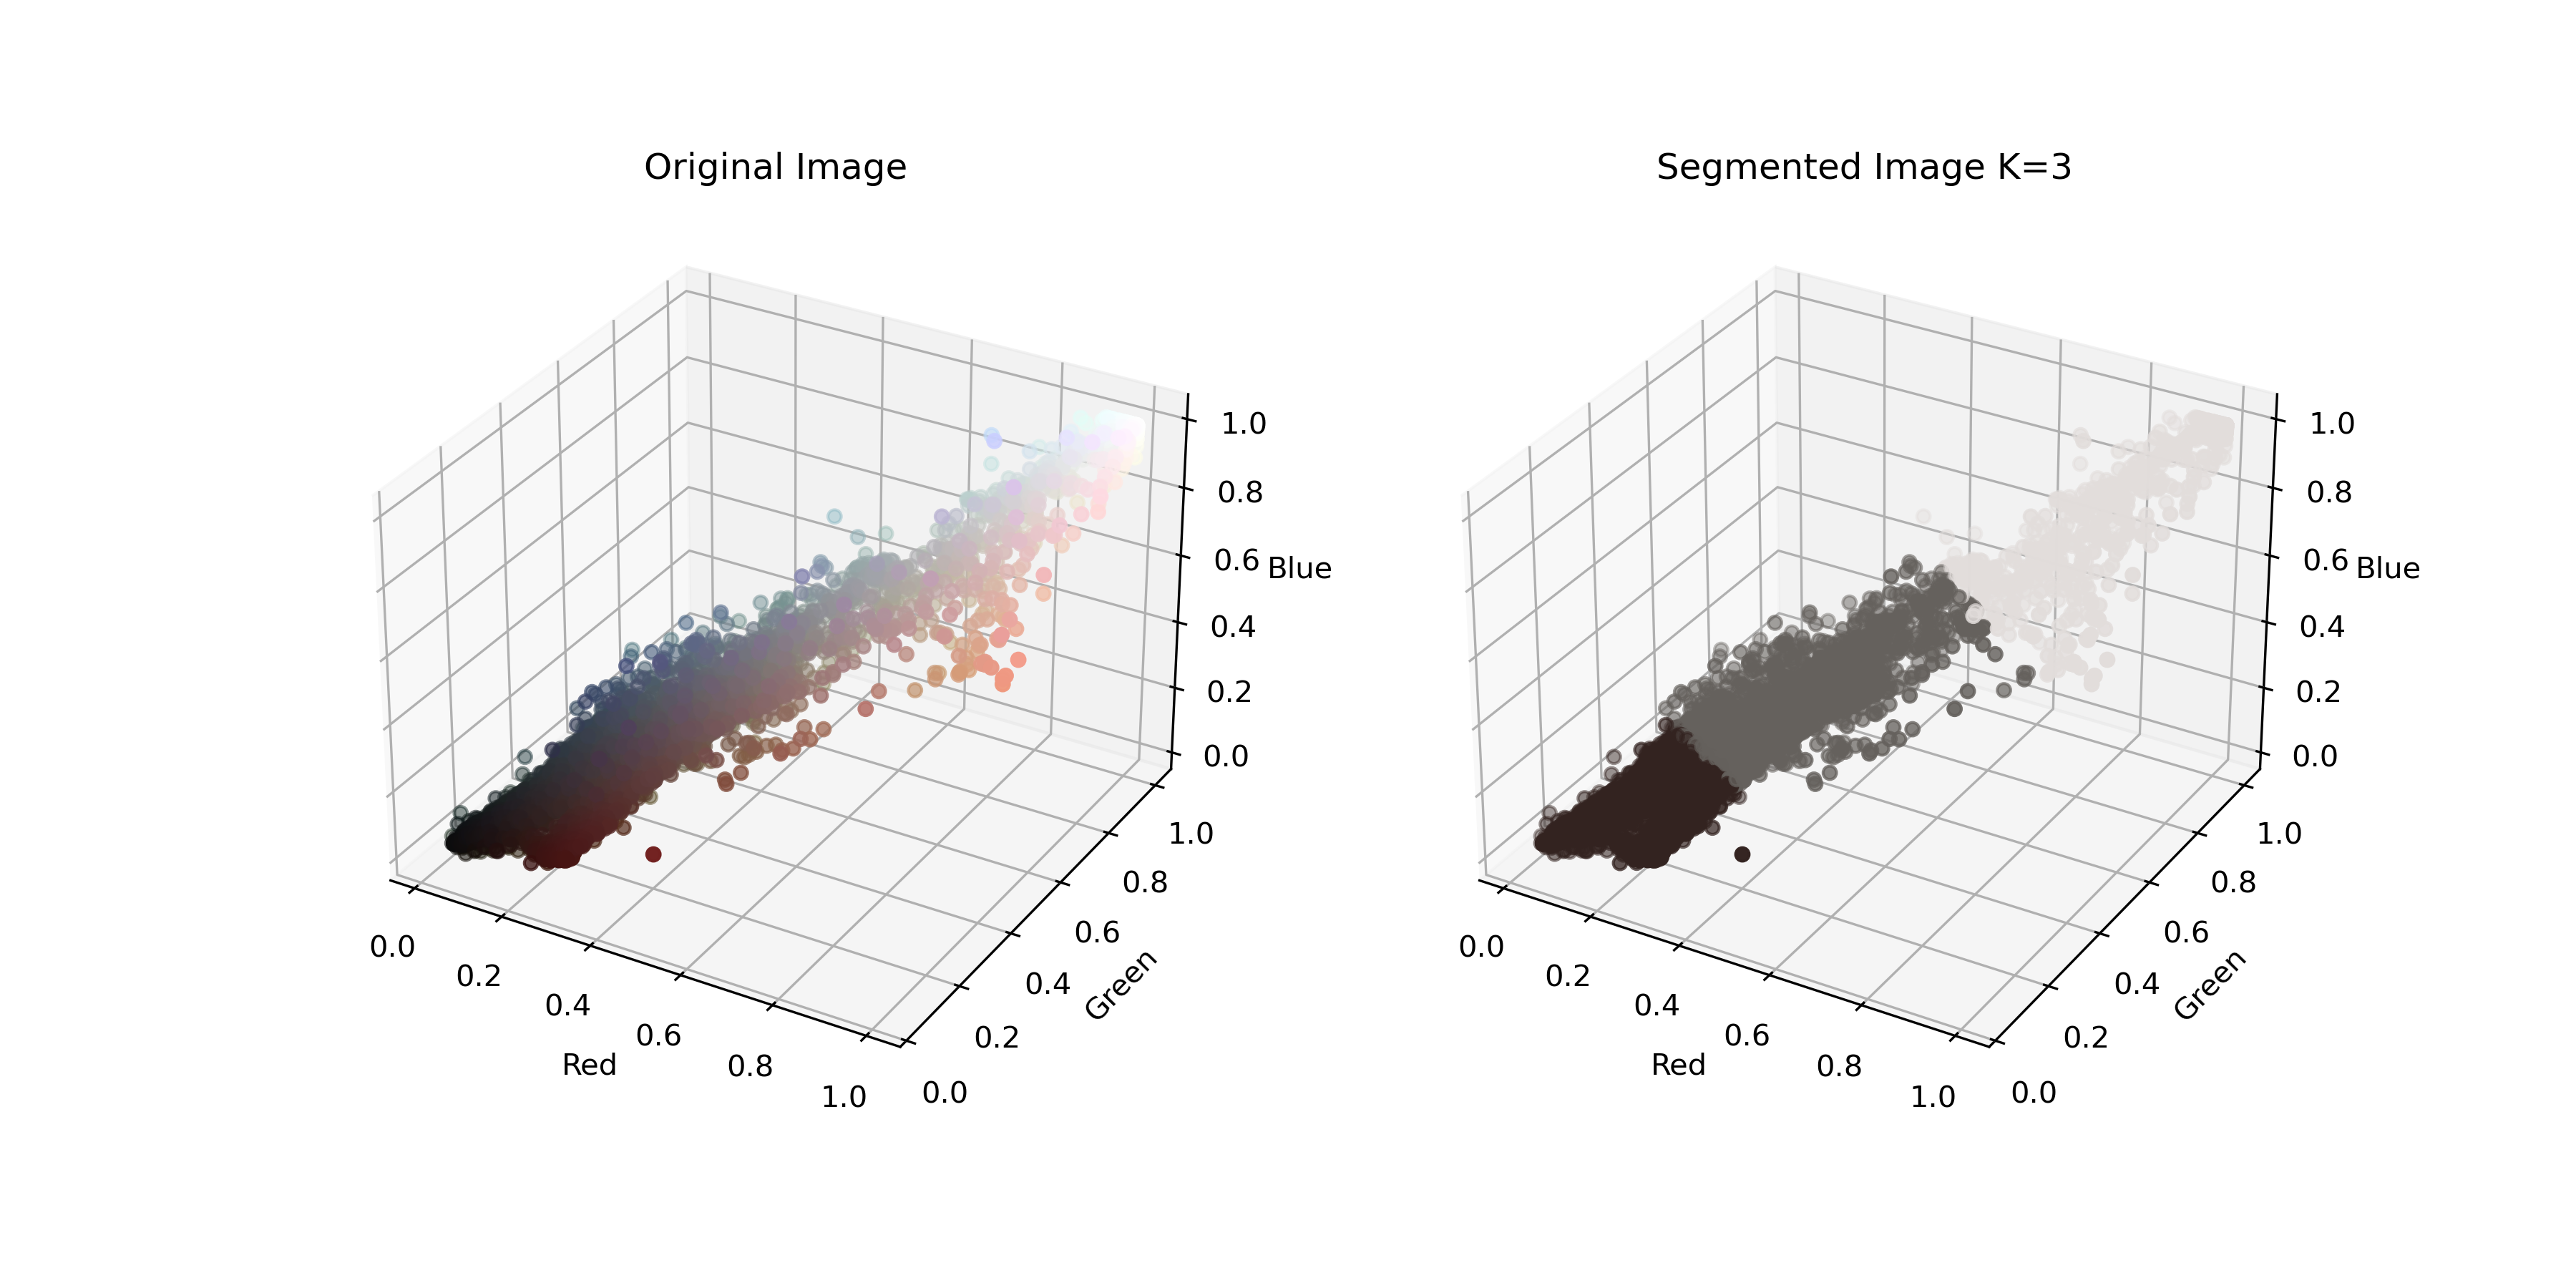
\includegraphics[width=3in]{image/scatter_3.png}
\caption{RGB空间点集}
\end{figure}

\begin{figure}[H]
\centering
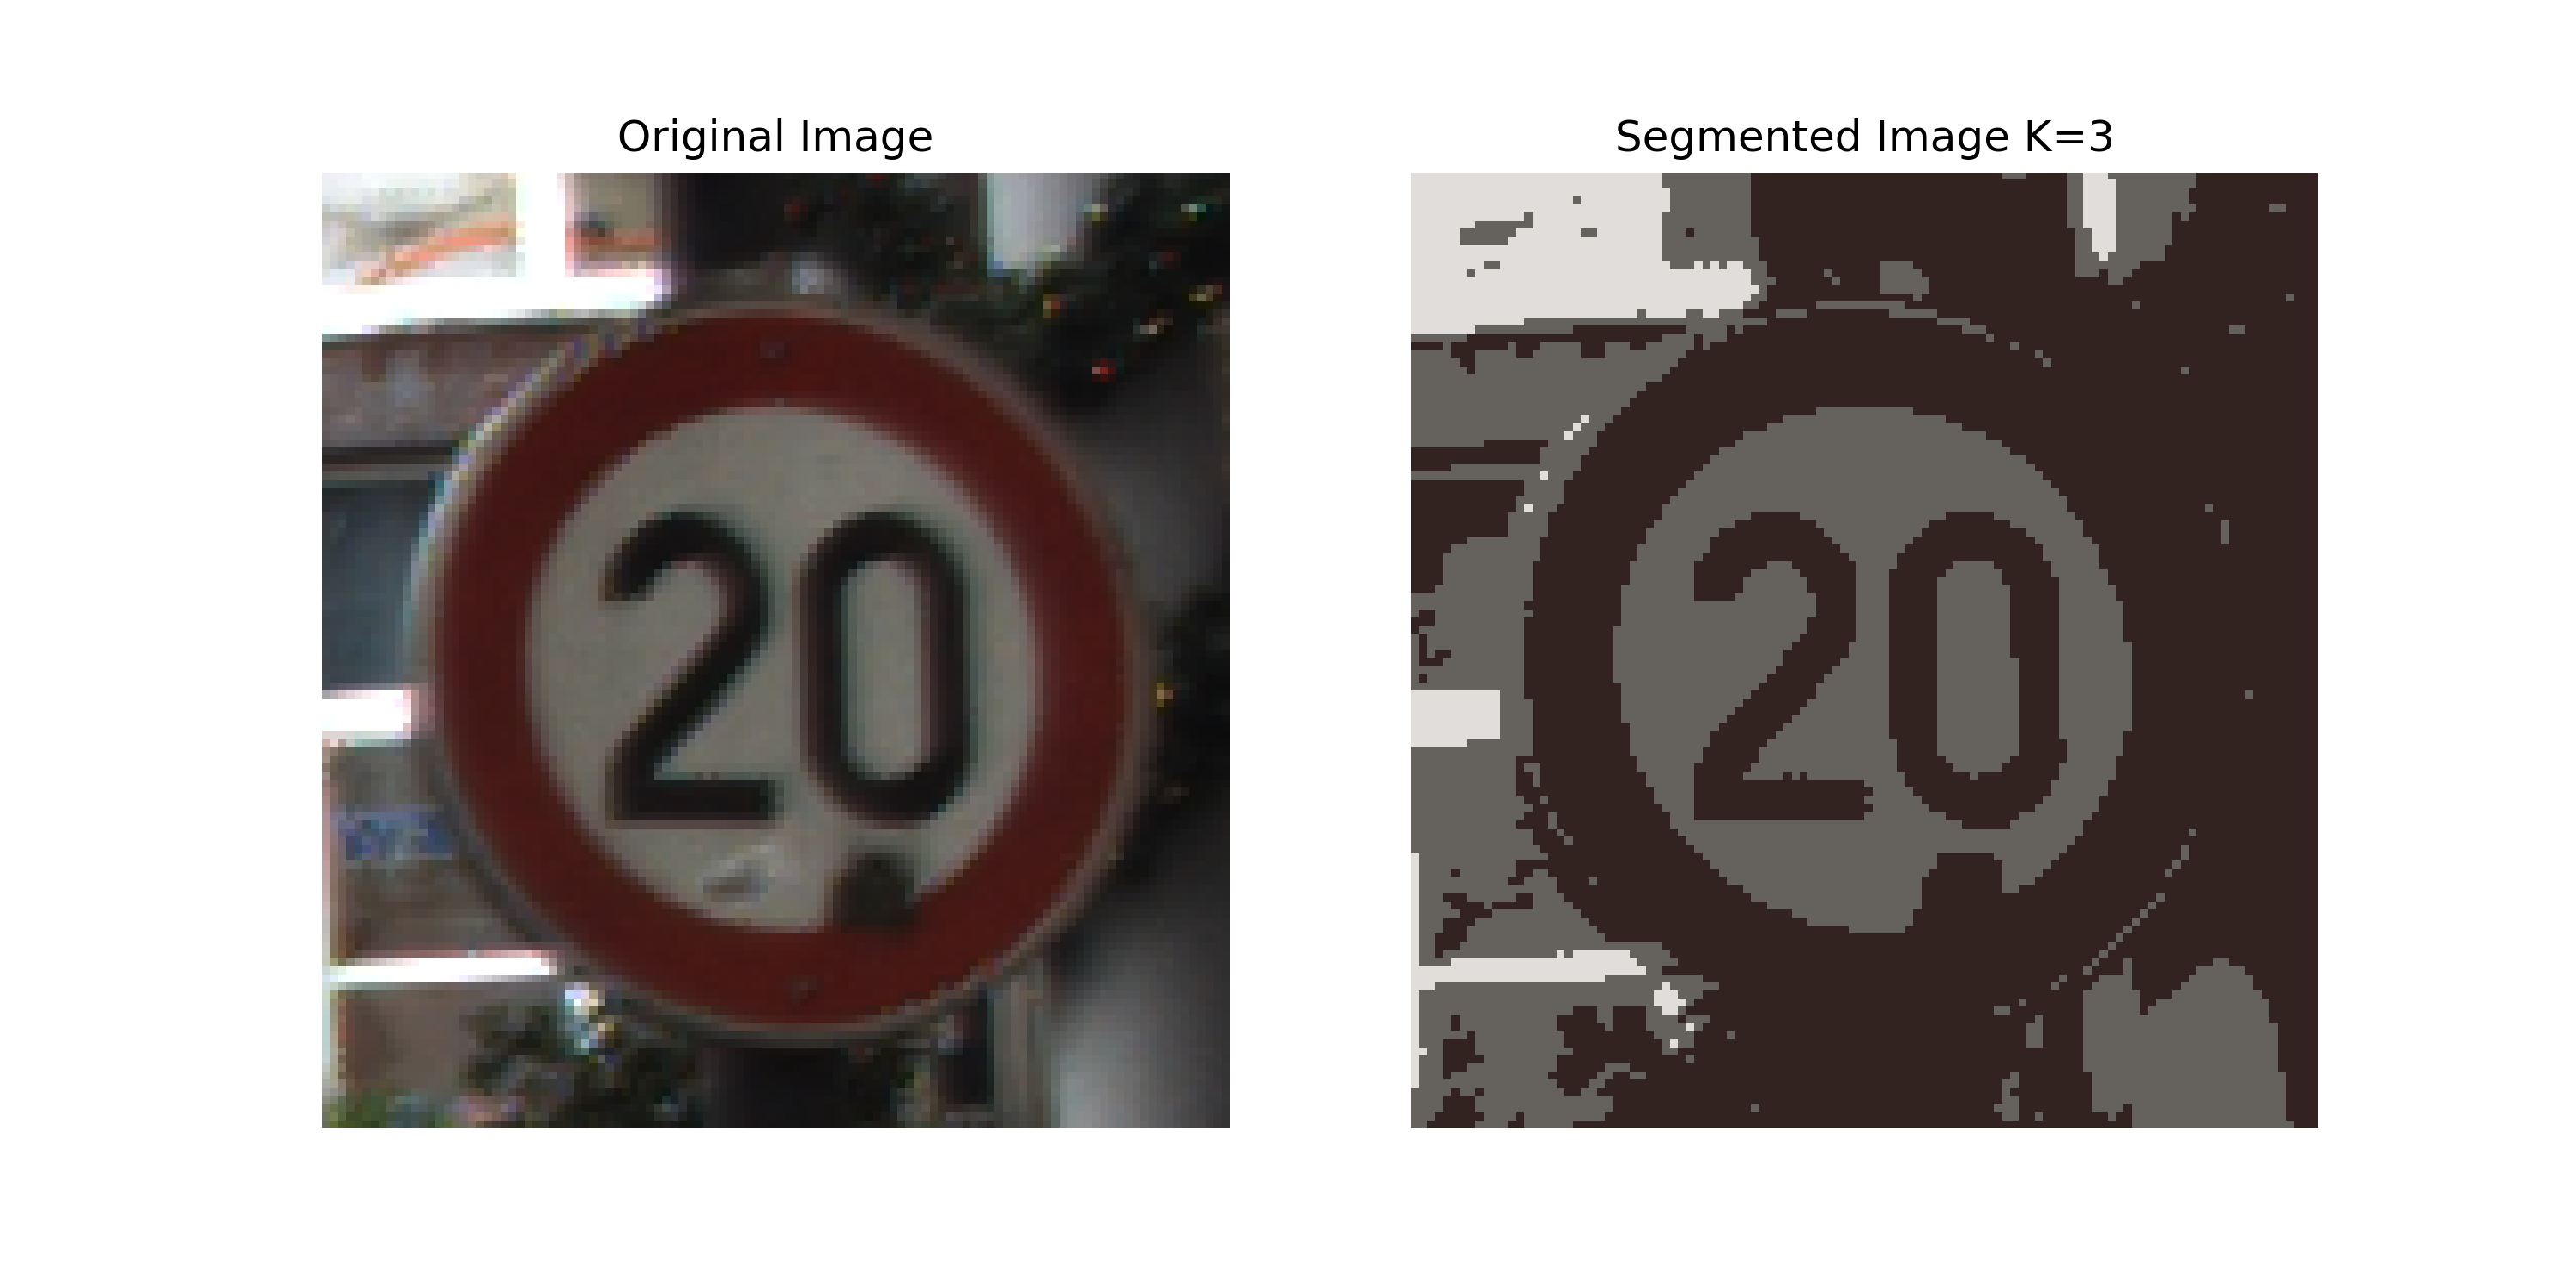
\includegraphics[width=3in]{image/Image_3.png}
\caption{图像分割结果}
\end{figure}

\begin{figure}[H]
\centering
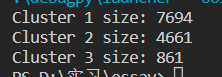
\includegraphics[width=3in]{image/K3.png}
\caption{每个聚类的像素数量}
\end{figure}

K = 6 时结果显示:

\begin{figure}[H]
\centering
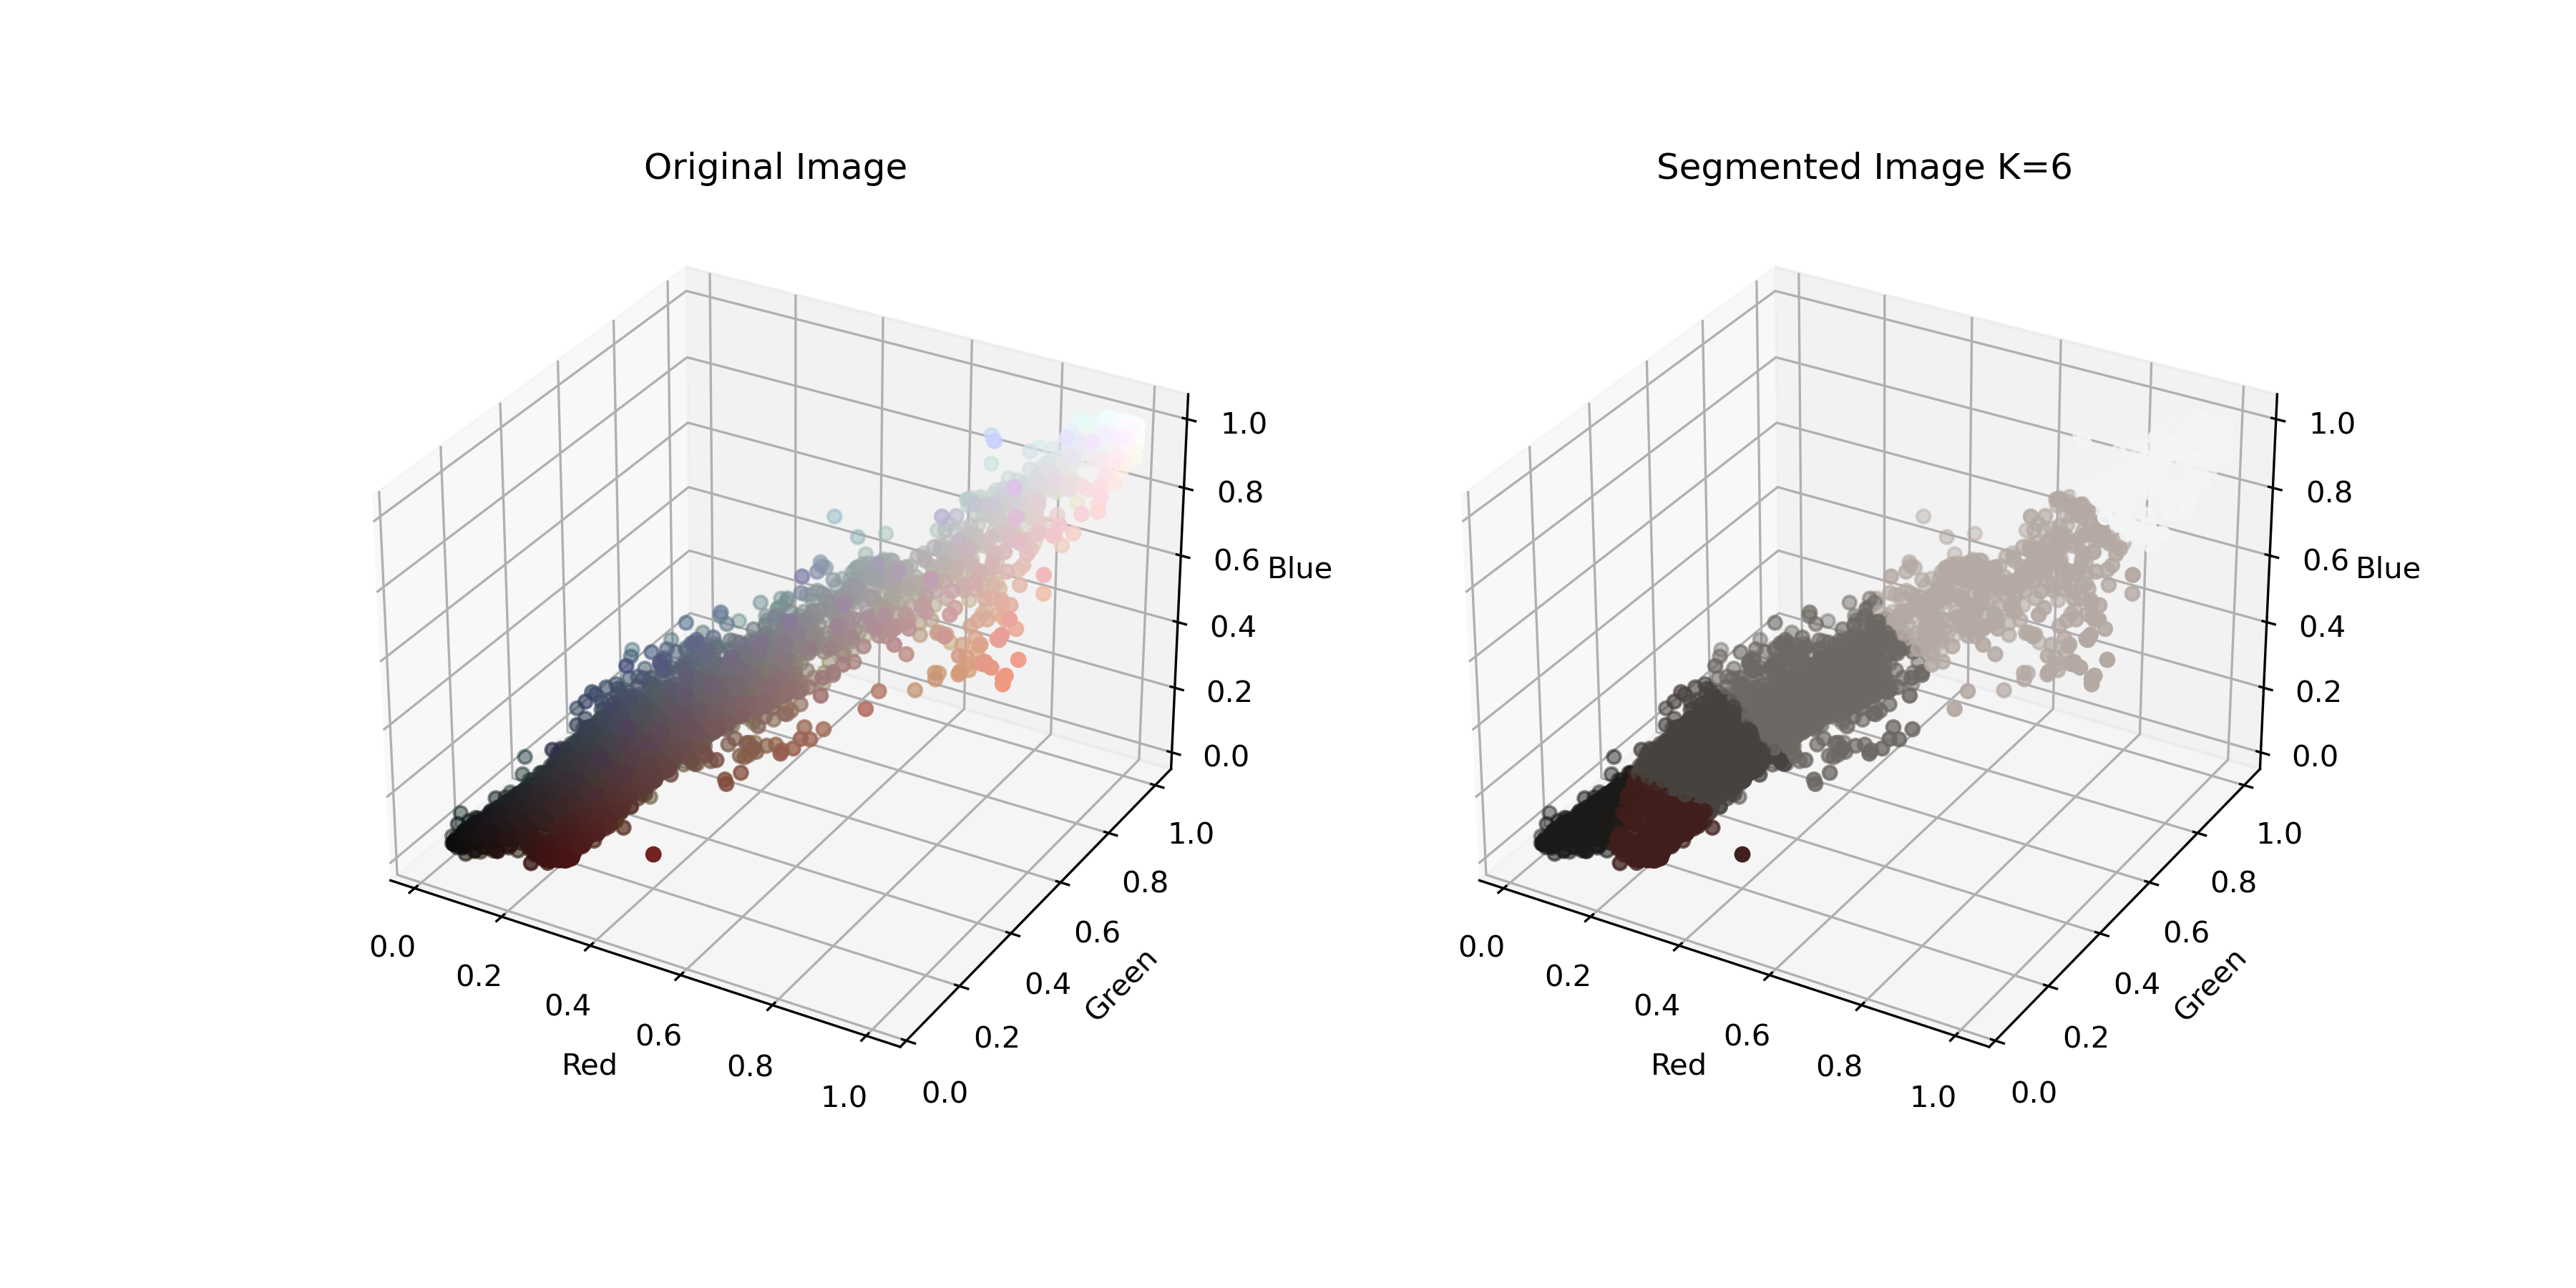
\includegraphics[width=3in]{image/scatter_6.png}
\caption{RGB空间点集}
\end{figure}

\begin{figure}[H]
\centering
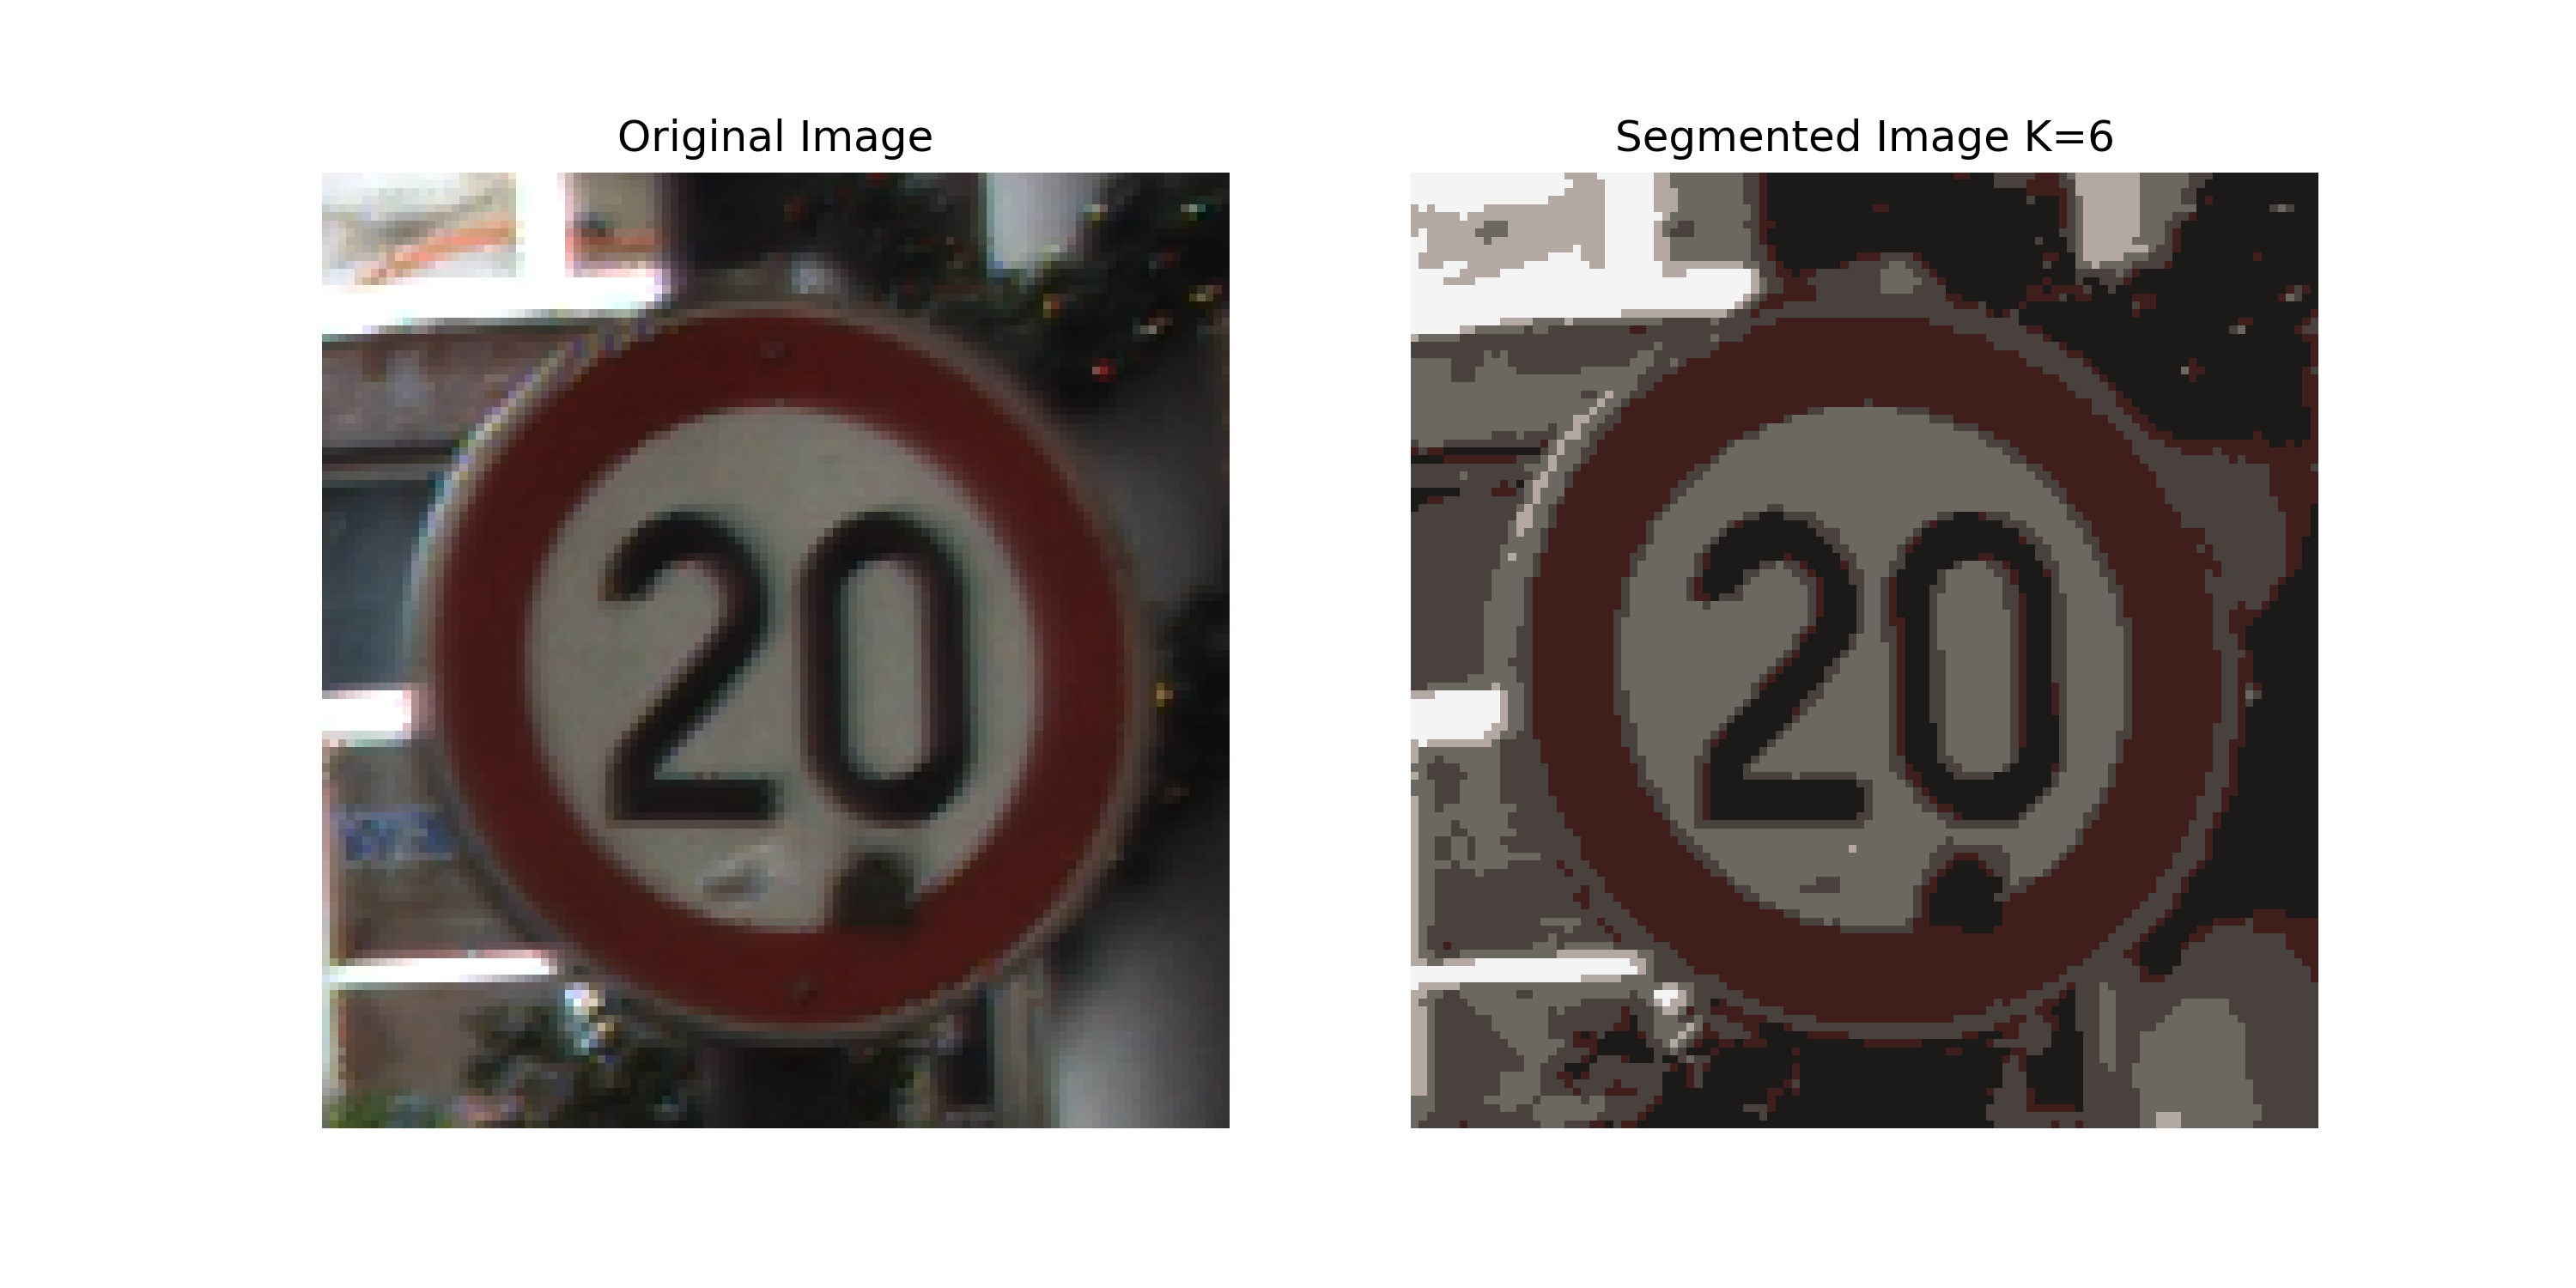
\includegraphics[width=3in]{image/Image_6.png}
\caption{图像分割结果}
\end{figure}

\begin{figure}[H]
\centering
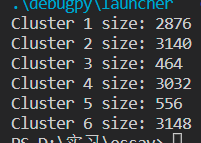
\includegraphics[width=2.5in]{image/K6.png}
\caption{每个聚类的像素数量}
\end{figure}

从图4,图7中可以明显地看出分割的效果,以及K值选取不同而带来的不同的图像分割的粗细。在此基础上,实验选取K值取6时的聚类结果,计算其轮廓系数(Silhouette Coefficient),Calinski-Harabasz指数(Calinski-Harabasz Index),Dunn指数(Dunn Index),进行定量分析以评估图像分割结果的质量。输出如下:

Average Silhouette Coefficient: 0.5396894

Calinski-Harabasz Index: 53952.501572485366

Dunn Index: 0.569386926380607

轮廓系数用于度量聚类的紧密度和分离度,取值范围为[-1, 1],越接近1表示聚类结果越好。在本实验中,平均轮廓系数为0.5396894,聚类结果相对较好。Calinski-Harabasz指数同样用于度量聚类的紧密度和分离度,取值越大表示聚类结果越好。Dunn指数用于度量聚类结果中最近聚类之间的距离和不同聚类之间的距离,取值越大表示聚类结果越好。

通过上述聚类性能指标的计算结果,可以定量评估聚类结果的质量,较高的轮廓系数、Calinski-Harabasz指数和Dunn指数表明本实验中的图像分割结果相对较好。此外根据各个聚类的像素数量,可以观察到不同聚类的大小差异较大,这可能反映了图像中不同区域的特点和分布情况。

\section{总结}

本实验深入探究了K\-means和Mean Shift聚类方法的原理,并在交通信号灯数据集上进行了实验分析。通过定量评估聚类结果的质量,对比分析了不同聚类方法的效果。然而,聚类效果仍有待提升,后续会进一步尝试不同的聚类算法、特征工程方法和数据预处理方式,以找到更好的聚类方案,继续研究和改进聚类方法在图像分析和处理中的应用。


\begin{thebibliography}{1}

\bibitem{ams}
{\it{数据分析-聚类}}, {\it{ITLiu\_JH}}, {\it{CSDN}}, {\it{2022年03月29日}}, \url{https://blog.csdn.net/it_liujh/article/details/123308992}

\bibitem{ams}
{\it{聚类模型评价(python实现)}}, {\it{三猫后端}}, {\it{WeChat official account}}, {\it{2019年08月21日}}, \url{https://mp.weixin.qq.com/s?__biz=MzAwNTIyMDU3NA==&mid=2648492629&idx=1&sn=756fcf111956e055c242057b7e65ee92&chksm=83379be4b44012f2b2485559c877c2272b40705c4622a029bfbba5fb9e74f200df7b0797c79b&token=1335603314&lang=zh_CN#rd}

\bibitem{ams}
{\it{chatgpt}}, May 24 Version

\end{thebibliography}



\end{document}


